\documentclass[8.5pt,twoside,twocolumn]{article}
\oddsidemargin -1.2cm
\evensidemargin -1.2cm
\textwidth 18cm
\headheight 1.0in
\topmargin -3.5cm
\textheight 22cm
\usepackage[super,sort&compress,comma]{natbib} 
%\usepackage{mhchem}
\usepackage{amsmath}
\usepackage{times,mathptmx}
% \usepackage{times}
% feel free not to use mathptmx if it causes difficulties
\usepackage{sectsty}
\usepackage{balance} 

\usepackage{graphicx} %eps figures can be used instead
\usepackage{lastpage}
\usepackage[format=plain,justification=raggedright,singlelinecheck=false,font=small,labelfont=bf,labelsep=space]{caption} 
\usepackage{fancyhdr}
\pagestyle{fancy}

\usepackage{SIunits}

\usepackage{pgfplots}
\usepgfplotslibrary{external}
\usepgfplotslibrary{groupplots}
\usetikzlibrary{positioning}
\usetikzlibrary{plotmarks}
\usetikzlibrary{patterns}
\usetikzlibrary{matrix}
\tikzexternalize
\tikzsetexternalprefix{fig_}
\tikzset{external/force remake=false}
\tikzset{every mark/.append style={scale=0.8}}
\pgfplotsset{every axis/.append style={small}}

\begin{document}

\thispagestyle{plain}
\fancypagestyle{plain}{
\fancyhead[L]{
\includegraphics[height=8pt]{headers/LH}}
\fancyhead[C]{\hspace{-1cm}
\includegraphics[height=20pt]{headers/CH}}
\fancyhead[R]{
\includegraphics[height=10pt]{headers/RH}\vspace{-0.2cm}}
\renewcommand{\headrulewidth}{1pt}}
\renewcommand{\thefootnote}{\fnsymbol{footnote}}
\renewcommand\footnoterule{\vspace*{1pt}% 
\hrule width 3.4in height 0.4pt \vspace*{5pt}} 
\setcounter{secnumdepth}{5}



\makeatletter 
\def\subsubsection{\@startsection{subsubsection}{3}{10pt}{-1.25ex plus -1ex minus -.1ex}{0ex plus 0ex}{\normalsize\bf}} 
\def\paragraph{\@startsection{paragraph}{4}{10pt}{-1.25ex plus -1ex minus -.1ex}{0ex plus 0ex}{\normalsize\textit}} 
\renewcommand\@biblabel[1]{#1}            
\renewcommand\@makefntext[1]% 
{\noindent\makebox[0pt][r]{\@thefnmark\,}#1}
\makeatother 
\renewcommand{\figurename}{\small{Fig.}~}
\sectionfont{\large}
\subsectionfont{\normalsize} 

\fancyfoot{}
\fancyfoot[LO,RE]{\vspace{-7pt}
\includegraphics[height=9pt]{headers/LF}}
\fancyfoot[CO]{\vspace{-7.2pt}\hspace{12.2cm}
\includegraphics{headers/RF}}
\fancyfoot[CE]{\vspace{-7.5pt}\hspace{-13.5cm}
\includegraphics{headers/RF}}
\fancyfoot[RO]{\footnotesize{\sffamily{1--\pageref{LastPage} ~\textbar  \hspace{2pt}\thepage}}}
\fancyfoot[LE]{\footnotesize{\sffamily{\thepage~\textbar\hspace{3.45cm} 1--\pageref{LastPage}}}}
\fancyhead{}
\renewcommand{\headrulewidth}{1pt} 
\renewcommand{\footrulewidth}{1pt}
\setlength{\arrayrulewidth}{1pt}
\setlength{\columnsep}{6.5mm}
\setlength\bibsep{1pt}

\twocolumn[
  \begin{@twocolumnfalse}
\noindent\LARGE{\textbf{Quantitative localisation and sizing of polydisperse colloids from confocal microscopy images}}
\vspace{0.6cm}

\noindent\large{\textbf{Mathieu Leocmach\textit{$^{a}$} and
Hajime Tanaka$^{\ast}$\textit{$^{a}$}}}\vspace{0.5cm}
%Please note that \ast indicates the corresponding author(s) but no footnote text is required. 


\noindent\textit{\small{\textbf{Received Xth XXXXXXXXXX 20XX, Accepted Xth XXXXXXXXX 20XX\newline
First published on the web Xth XXXXXXXXXX 200X}}}

\noindent \textbf{\small{DOI: 10.1039/b000000x}}
\vspace{0.6cm}
%Please do not change this text.

\vspace{0.5cm}
 \end{@twocolumnfalse}
  ]

\tikzset{external/force remake=false}
\tikzsetnextfilename{localise}
\begin{figure*}
	\centering
	\begin{tikzpicture}[
		pic3d/.style={inner sep=0}, %
		lab/.style={above right, text height=0.8em, text depth=0.2em, font=\Large\bfseries}%
		]%
		\node[pic3d] (m3d) {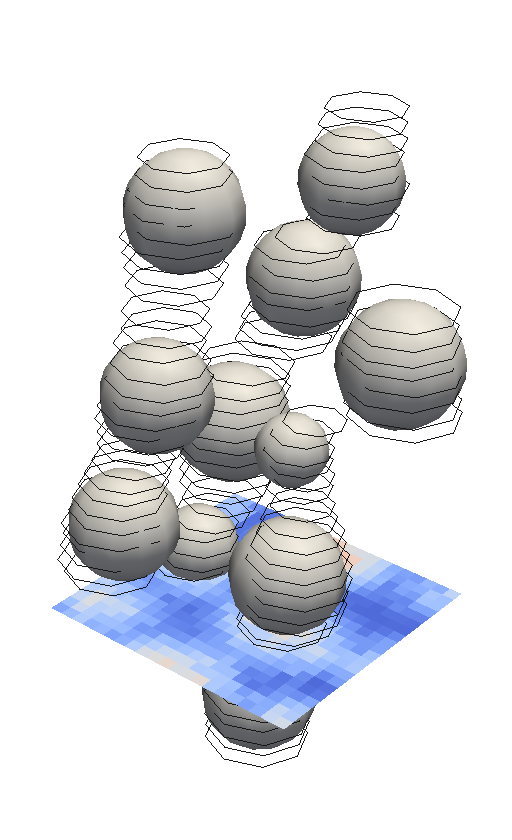
\includegraphics[width=0.28\textwidth]{comp2D3D_crop}};
		\node[lab] at (m3d.south west) {a};
		\node [pic3d, right] at (m3d.east) (m2d) {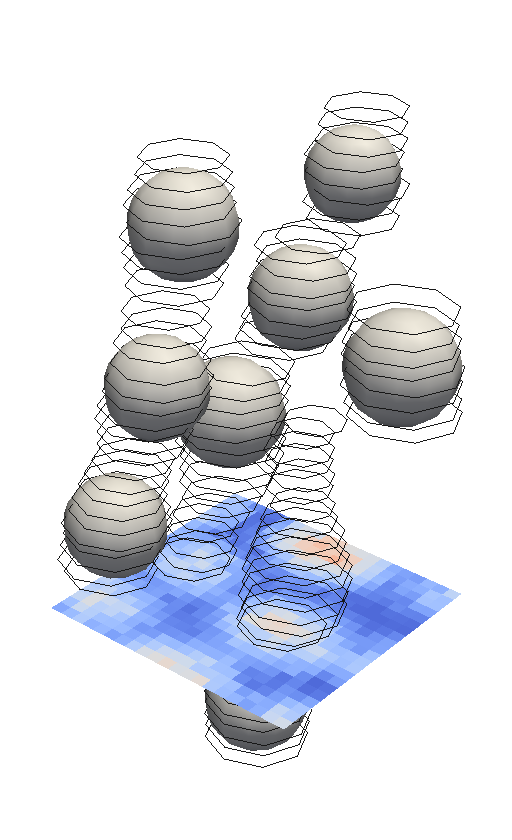
\includegraphics[width=0.28\textwidth]{comp2D_reconstructed_crop}};
		\node[lab] at (m2d.south west) {b};
		\node [pic3d, below right] at (m2d.north east) (cg20) {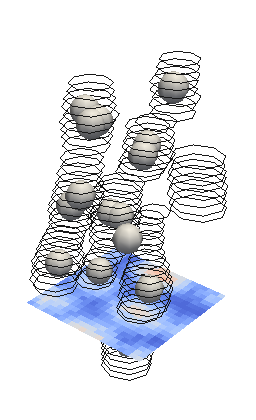
\includegraphics[width=0.14\textwidth]{comp3D_monoscale_r20_crop}};
		\node[lab] at (cg20.south west) {c};
		\node [pic3d, right] at (cg20.east) (cg25) {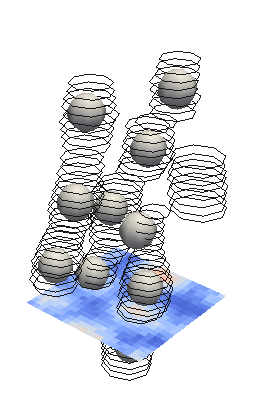
\includegraphics[width=0.14\textwidth]{comp3D_monoscale_r25_crop}};
		\node[lab] at (cg25.south west) {d};
		\node [pic3d, right] at (cg25.east) (cg30) {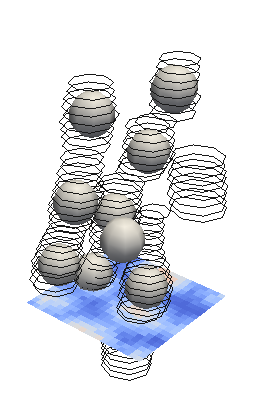
\includegraphics[width=0.14\textwidth]{comp3D_monoscale_r30_crop}};
		\node[lab] at (cg30.south west) {e};
		\node [pic3d, above right] at (m2d.south east) (cg35) {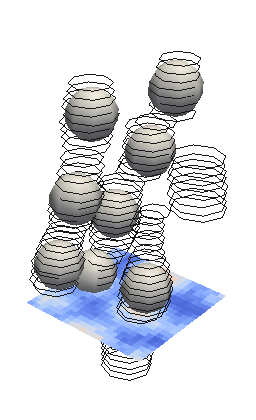
\includegraphics[width=0.14\textwidth]{comp3D_monoscale_r35_crop}};
		\node[lab] at (cg35.south west) {f};
		\node [pic3d, right] at (cg35.east) (cg40) {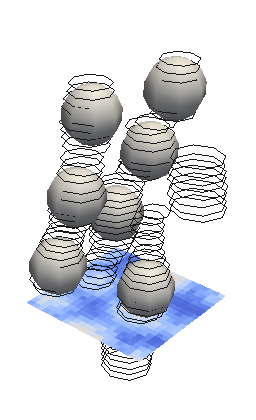
\includegraphics[width=0.14\textwidth]{comp3D_monoscale_r40_crop}};
		\node[lab] at (cg40.south west) {g};
		\node [pic3d, right] at (cg40.east) (cg45) {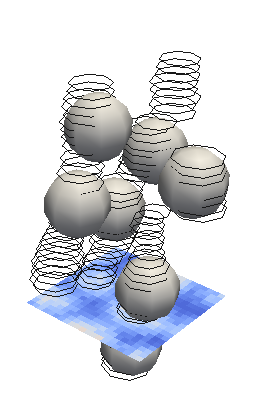
\includegraphics[width=0.14\textwidth]{comp3D_monoscale_r45_crop}};
		\node[lab] at (cg45.south west) {h};
	\end{tikzpicture}
	\caption{\textbf{Visualisation of the results of various tracking methods for the same portion of image.} \textbf{a} Multiscale 3D tracking. \textbf{b} Reconstruction from 2D tracking. \textbf{c-h} Crocker and Grier in 3D with blurring radius increasing from \unit{2}{px} to \unit{4.5}{px} by steps of \unit{0.5}{px}. The circles on each picture are the result of 2D multiscale tracking of each XY slice of the 3D pictures. Sphere are displayed with radii determined by the tracking methods in \textbf{a-b}, and equal to the blurring radius for \textbf{c-h}.}
	\label{fig:localise}
\end{figure*}

\tikzset{external/force remake=false}
\tikzsetnextfilename{sizing}
\begin{figure}
	\centering
	\begin{tikzpicture}[lab/.style={anchor=south west, text height=0.8em, text depth=0.2em, font=\Large\bfseries}]
	\begin{groupplot}[%
		group style={
				group name=ro,
				group size=1 by 2,%
				%horizontal sep=0.0075\textwidth,
				%vertical sep=0.0075\textwidth,
				},%
		width=0.925\columnwidth,%
		height=0.5\columnwidth,%
		y label style={align=center, text width=0.5\columnwidth},%
		]
	\nextgroupplot[%
		xmin=2, xmax=6, xlabel={Detected radius [px]},%
		ymin=0, ymax=20,%
		ylabel={Position of the first peak of $g_R(r)$ [px]},
		]
		\addplot+[black,forget plot, no marks, domain=2:6] {3*x};
		\addplot+[black,only marks, mark=o] file {rdf_peak_pos_radius};
	
	\nextgroupplot[%
		xmin=0, xmax=60, 
		xlabel={Time [h]},%
		%ymin=0, ymax=20,%
		ylabel={Real-to-optical\\ size ratio},
		]
		\addplot+[red,only marks, mark=+] table[x expr=12*\coordindex/60, y index=0] {ro_ratio};
		\addplot+[black,very thick, no marks, domain=0:60] {0.00125333*x+1.48757};
		
	\end{groupplot}
	\node[lab] at (ro c1r1.outer south west) {a};
	\node[lab] at (ro c1r2.outer south west) {b};
	
	\begin{axis}[%
		name=hist,
		anchor=outer north west,
		at={(ro c1r2.outer south west)},
		width=0.6\columnwidth, height=0.5\columnwidth,%
		%scale only axis,
		xlabel={Diameters [$\micro\metre$]},%
		xmin=1, xmax=5,
		axis y line*=left,
		ymin=0, ytick=\empty,%
		ylabel={Size distribution},%
		ylabel near ticks,
		]
		\addplot[ybar, ybar interval, gray!50, fill=gray!50] file {SEM_size_distrib.txt} \closedcycle;
	\end{axis}
	\begin{axis}[%
		name=hist2,
		at={(hist.south west)},
		width=0.6\columnwidth, height=0.5\columnwidth,%
		xmin=1, xmax=5,
		axis y line*=right,
		ymin=0, ytick=\empty,%
		no marks,%
		]
		\addplot+[dashed] table[x expr ={2*\thisrow{r}}, y=all] {all_ico_icongb_mrco_X.rdist};
		\addplot table [x expr ={2*\thisrow{r}/1.25}, y index=1] {all_ico_icongb_mrco_X.rdist};
		\draw[->, ultra thick] (axis cs:3.15,3) -- (axis cs: 3.9, 3);% node[right)] {swelling};
	\end{axis}
	\node[lab] at (hist.outer south west) {c};
	
	\begin{axis}[%
		name=srdf,
		anchor=north east,
		at={(ro c1r2.below south east)},
		width=0.5\columnwidth, height=0.5\columnwidth,%
		xmin=0, xmax=1.5,%
		xlabel ={$r/\sigma_\text{peak}$, $\hat{r}$},%
		ymin=0,%
		ylabel=$g(r)$, ylabel near ticks,%
		no marks,%
		legend style={legend pos=north west}
		]
		\addplot+[dashed] file {yon6.rdf};
		\addplot file {yon6.srdf};
		\legend{$g(r)$, $g(\hat{r})$};
	\end{axis}
	\node[lab] at (srdf.outer south west) {d};
	
	
	
	
	\end{tikzpicture}
	\caption{\emph{In situ} sizing of colloids in a glass. (a) Position of the first peak of the partial $g_R(r)$ function of the optical radius $R$. Solid line corresponds to a real-to-optical size ratio of $1.5$. (b) Time dependence of the real-to-optical size ratio. Solid line is a linear fit. (c) Size distribution estimated by our algorithm (dashed line). Comparison with the estimation from \textsc{sem} of only $140$ dry particles (steps) is possible once $25\%$ of swelling is taken into account (full line). (d) First peak of the radial distribution function with (full line) and without (dashed) the individual sizes data.}
	\label{fig:sizing}
\end{figure}


\tikzset{external/force remake=false}
\tikzsetnextfilename{deconv}
\begin{figure*}
	\centering
	\begin{tikzpicture}[
		lab/.style={above right, text height=0.8em, text depth=0.2em, font=\Large\bfseries}%
		]%
		\begin{groupplot}[%
		group style={
				group name=pics,
				group size=4 by 1,%
				horizontal sep=0.0075\textwidth,
				vertical sep=0.0075\textwidth,
				},%
		width=0.225\textwidth,%
		height=0.2475\textwidth,%
		xmin=0,xmax=50,ymin=0,ymax=55,%
		axis lines=none,%
		scale only axis=true,%
		point meta=explicit symbolic,%
		scatter/@pre marker code/.code={%
        	\pgfmathparse{10*\pgfplotspointmetatransformed*\pgfplotsunitxlength}%
        	%\pgfplotstransformcoordinatex{\pgfplotspointmetatransformed}
            \def\markopts{mark=o,black,mark size=\pgfmathresult}%
            \expandafter\scope\expandafter[\markopts]
            },%
        scatter/@post marker code/.code={\endscope} 
		]
		\nextgroupplot
			\addplot graphics [xmin=0,xmax=50,ymin=0,ymax=55]{Zelong_original};
			\node[lab] at (rel axis cs:0,0){a};
		\nextgroupplot
			\addplot graphics [xmin=0,xmax=50,ymin=0,ymax=55]{Zelong_blurred};
			\addplot+[only marks, scatter] table [x index=1, y expr={55-\thisrowno{2}}, meta index=3] {Z_elong.xyz};
			\node[lab] at (rel axis cs:0,0){b};
		\nextgroupplot
			\addplot graphics [xmin=0,xmax=50,ymin=0,ymax=55]{Zelong_deconvolved};
			\addplot+[only marks, scatter] table [x index=1, y expr={55-\thisrowno{2}}, meta index=3] {Z_elong_deconv.xyz};
			\node[lab] at (rel axis cs:0,0){c};
		\nextgroupplot
			\node[lab] at (rel axis cs:0,0){d};
		\end{groupplot}
		\begin{axis}[%
			at={(pics c4r1.south west)},%
			anchor=outer south west,
			width=0.225\textwidth,%
			height=0.28\textwidth,%
			xlabel = {$r$ [$\micro\metre$]}, ylabel={$g(r)$},%
			xlabel near ticks, ylabel near ticks,
			xmin=0,xmax=4,ymin=0,%
			no marks,%
			]
			\addplot file {cp0.34.rdf};
			\addplot+[dashed] file {cp0.34_deconv.rdf};
		\end{axis}
	\end{tikzpicture}
	\caption{\textbf{Deconvolution.} Detail of the same $YZ$ slice of \textbf{a} original confocal image, \textbf{b} previous blurred by $\sigma_0=1.6$, \textbf{c} previous deconvolved by measured kernel (see text). Circles indicate the tracked particles position and size when using whether \textbf{b} or \textbf{c} as first Gaussian layer $G_0$. All three centres are in the slice $\pm \unit{0.5}{px}$. \textbf{d} Radial distribution function of sticky spheres (blue) without and (red dash) with deconvolution.}
	\label{fig:deconv}
\end{figure*}


\tikzset{external/force remake=false}
\tikzsetnextfilename{perfect}
\begin{figure}
	\centering
	\begin{tikzpicture}[
		lab/.style={anchor=south west, text height=0.8em, text depth=0.2em, font=\Large\bfseries}%
		]%
	\pgfplotsset{cycle list name=black white, clip marker paths=true,}
	\begin{axis}[%
		name=size,
		width=0.5\columnwidth,%
		height=0.5\columnwidth,%
		xlabel={Input radius}, ylabel={Output radius},%
		xmin=0, xmax=15, ymin=0, ymax=15,%
		extra x ticks={3.47}, extra x tick labels={}, extra tick style={grid=major},%
		%ytick={2,4,...,14},
		axis background/.style={fill=white},%
		]
		\addplot+[only marks, mark size=0.5, mark=o] table [x index=0, y expr ={\thisrowno{1}}] {multiscale_relative_sizes.out};
		\addplot+[no marks, domain=1.5:14] {x};
	\end{axis}
	\node[lab] at (size.outer south west) {a};
	\begin{axis}[%
		name=errorsize,
		at={(0.5\columnwidth,0)},%
		width=0.5\columnwidth,%
		height=0.5\columnwidth,%
		xlabel={Input radius (px)}, ylabel={$R$ relative error (\%)},%
		xmin=0, xmax=15,%
		extra x ticks={3.47}, extra x tick labels={}, extra tick style={grid=major},%
		extra y ticks={0}, extra y tick labels={},%
		ylabel near ticks,
		]
		\addplot table [x index=0, y expr ={100*(\thisrowno{1}/\thisrowno{0}-1)}] {multiscale_relative_sizes.out};
	\end{axis}
	\node[lab] at (errorsize.outer south west) {b};
		
	
	\begin{axis}[%
		name=dist_er,
		at={(0,-0.45\columnwidth)},%
		height=0.5\columnwidth,%
		width=\columnwidth,%
		xlabel={$r_{ij}$ (px)}, ylabel={$r_{ij}$ error (\unit{0.01}{px})},%
		xmin=8, xmax=18, xtick={8,...,17},%
		extra tick style={grid=major},%
		extra y ticks={0}, extra y tick labels={}
		]
		\addplot table [x index=0, y expr ={(\thisrowno{2}-\thisrowno{1}-\thisrowno{0})*100}] {close_neighbours3D.out};
		\draw (axis cs:12,-6) circle[radius=0.03\textwidth] (axis cs:16,-6) circle[radius=0.03\textwidth];
		\draw[dashed] (axis cs:12,-6) -- (axis cs:12,-9) (axis cs:16,-9) -- (axis cs:16,-6);
		\draw[<->] (axis cs:12,-9) -- (axis cs:16,-9) node[midway, above] {$r_{ij}$};
		\draw[->] (axis cs:11.05,-6) -- +(0,0.03\textwidth,0) node[midway, left] {\unit{4}{px}};
		\draw[->] (axis cs:16.95,-6) -- +(0,0.03\textwidth,0) node[midway, right] {\unit{4}{px}};
		\draw[->, very thick] (axis cs:16,-6) -- (axis cs:14,-6);
	\end{axis}
	\node[lab] at (dist_er.outer south west) {c};
	
	\begin{axis}[%
		name=near_R,
		at={(0,-0.9\columnwidth)},%
		height=0.5\columnwidth,%
		width=\columnwidth,%
		xlabel={$r_{ij}$ (px)}, ylabel={$R$ (px)},%
		xmin=8, xmax=18, xtick={8,...,17},%
		extra tick style={grid=major},%
		extra y ticks={4}, extra y tick labels={},%
		legend style={legend pos=south east}
		]
		\addplot table [x index=0, y index=4] {close_neighbours3D.out};
		\addplot+[mark=square] table [x index=0,y index=6] {close_neighbours3D.out};
		\legend{No correction, One iteration};
	\end{axis}
	\node[lab] at (near_R.outer south west) {d};
	
	\begin{axis}[%
		name=finite,
		at={(0,-1.35\columnwidth)},%
		height=0.5\columnwidth,%
		width=\columnwidth,%
		area legend,
		const plot, no marks,%
		xlabel={$R$ (px)}, ylabel={Size distribution},%
		%xmin=8, xmax=18,%
		extra tick style={grid=major},%
		extra x ticks={5.298}, extra x tick labels={},%
		ymin=0,%		
		legend style={legend pos=north west, cells={anchor=west}}
		]
		\addplot+[pattern=north west lines] file {john_exact_mono_large_init.hist} \closedcycle;
		\addplot+[gray, fill=gray, semitransparent] file {john_exact_mono_large_cor1.hist} \closedcycle;
		\addplot+[pattern=dots] file {john_exact_mono_large_cor2.hist};
		\legend{No correction, One iteration, Two iterations};
		\draw[decorate,decoration=brace] (axis cs:4.75, 200) -- (axis cs:5.05, 200) node[midway, above] {edges};
	\end{axis}
	\node[lab] at (finite.outer south west) {e};
	\end{tikzpicture}
	\caption{\textbf{Results from perfect images.} \textbf{a,b} Sizing of an isolated sphere. Left of the vertical line our algorithm uses a doubled image. \textbf{c} Localisation error and \textbf{d} sizing error function of the distance between two particles. Oscillations are due to off-lattice centre position. \textbf{e} Size distribution extracted from digitized configuration of 4000 monodisperse hard spheres at $0.50$ volume fraction (the vertical line indicates the input radius). The tail to the right is due to particles on the edges of the image who have fewer neighbours and thus are more `dilute'. \textbf{d} and \textbf{e} also show the effect of finite dilution correction up to convergence.}
	\label{fig:perfect}
\end{figure}


\tikzset{external/force remake}
\tikzsetnextfilename{size_struc}
\begin{figure}
	\centering
	\begin{tikzpicture}[
		lab/.style={above right, text height=0.8em, text depth=0.2em, font=\Large\bfseries}%
		]%
	\begin{groupplot}[%
		group style={
			group name=distrib,
			group size=1 by 2,
			},%
		width=\columnwidth,%
		height=0.5\columnwidth,%
		no marks,%
		xlabel={$R$ [$\micro\metre$]}, xmin=0.8, xmax=2.5,%
		ylabel={Size distribution}, ymin=0, ymax=12,%
		legend style={legend pos=north west},
		]
		\nextgroupplot
		\addplot[gray!50,fill=gray!50, area legend] table[x=r, y=all] {all_ico_icongb_mrco_X.rdist} \closedcycle;
		\addplot[dashed] table[x=r, y=mrco] {all_ico_icongb_mrco_X.rdist};
		\addplot[black] table[x=r, y=X] {all_ico_icongb_mrco_X.rdist};
		\legend{all, \textsc{mrco}, crystalline};
		
		\nextgroupplot
		\addplot[gray!50,fill=gray!50, area legend] table[x=r, y=all] {all_ico_icongb_mrco_X.rdist} \closedcycle;
		\addplot[dashed] table[x=r, y=ico] {all_ico_icongb_mrco_X.rdist};
		\addplot[black] table[x=r, y=icongb] {all_ico_icongb_mrco_X.rdist};
		\legend{all, ico. centre, ico. surf.};
	\end{groupplot}
	\node[lab, above right=0 of distrib c1r1.outer south west] {a};
	\node[lab, above right=0 of distrib c1r2.outer south west] {b};
	\end{tikzpicture}
	\caption{\textbf{Size distribution within local structures in a hard sphere colloidal glass.} \textbf{a} With increasing local crystalline order: all particles, MRCO particles ($0.4>Q_6>0.25$) and crystalline particles ($Q_6>0.4$). Crystalline ordered regions are less polydisperse. \textbf{b} Particles at the centre or on the surface of icosahedra ($w_6<-0.023$). A small central particle with large surface particles tend to stabilize icosahedra.}
	\label{fig:size_struc}
\end{figure}

\tikzset{external/force remake=false}
\tikzsetnextfilename{applications}
\begin{figure}
	\centering
	\begin{tikzpicture}[
		lab/.style={above right, text height=0.8em, text depth=0.2em, font=\Large\bfseries}%
		]%
		\begin{groupplot}[%
		group style={
			group size=2 by 1,
			horizontal sep=0.01\textwidth,
			},%
		width=0.48\columnwidth,%
		height=0.48\columnwidth,%
		axis lines=none,%
		scale only axis=true,%
		clip marker paths=true,%
		point meta=explicit symbolic,%
        scatter/@post marker code/.code={\endscope} 
		]
		\nextgroupplot[xmin=0,xmax=511,ymin=0,ymax=511,%
			scatter/@pre marker code/.code={%
        	\pgfmathparse{1.5*\pgfplotspointmetatransformed*\pgfplotsunitxlength}%
            \def\markopts{mark=o,blue,mark size=\pgfmathresult}%
            \expandafter\scope\expandafter[\markopts]
            },]
			\addplot graphics [xmin=0,xmax=511,ymin=0,ymax=511]{microfluidic.png};
			\addplot+[only marks, scatter] table [x index=0, y expr={511-\thisrowno{1}}, meta index=2] {microfluidic.xyr};
			\draw[ultra thick, red!50!white] (axis cs:25,490) -- (axis cs:125,490)  node[midway, below]{200\micro\metre};
			
		\nextgroupplot[xmin=0,xmax=1500,ymin=0,ymax=1500,%
			scatter/@pre marker code/.code={%
        	\pgfmathparse{0.15*\pgfplotspointmetatransformed*\pgfplotsunitxlength}%
            \def\markopts{mark=o,blue,mark size=\pgfmathresult}%
            \expandafter\scope\expandafter[\markopts]
            },]
			\addplot graphics [xmin=0,xmax=1500,ymin=0,ymax=1500]{llt.png};
			\addplot+[only marks, scatter] table [x index=0, y expr={1500-\thisrowno{1}}, meta index=2] {llt.xyr};
			\draw[ultra thick, red!50!white] (axis cs:75,1435) -- (axis cs:375,1435)  node[midway, below]{50\micro\metre};
		\end{groupplot}
	\end{tikzpicture}
	\caption{\textbf{Application of \textsc{sift} in 2D.} \textbf{a} Fluorescent droplets in a microfluidic device. \textbf{b} Nucleation under phase contrast microscope. The circles are the result of our algorithm.}
	\label{fig:applications}
\end{figure}

\tikzset{external/force remake=false}
\tikzsetnextfilename{small_expelled}
\begin{figure}
	\centering
	\begin{tikzpicture}[
		lab/.style={above right, text height=0.8em, text depth=0.2em, font=\Large\bfseries}%
		]%
		\matrix[matrix of nodes, inner sep=1pt] (a)%
		{%
			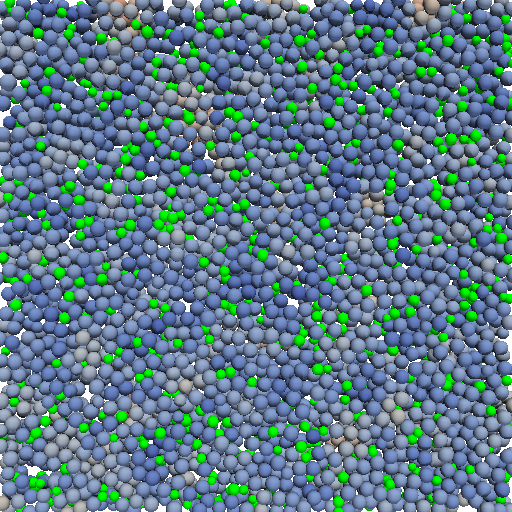
\includegraphics[width=0.29\columnwidth]{small_boo000.png} & %
			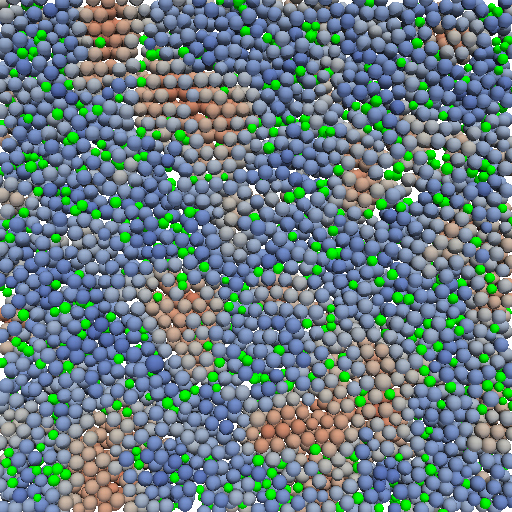
\includegraphics[width=0.29\columnwidth]{small_boo060.png} & %
			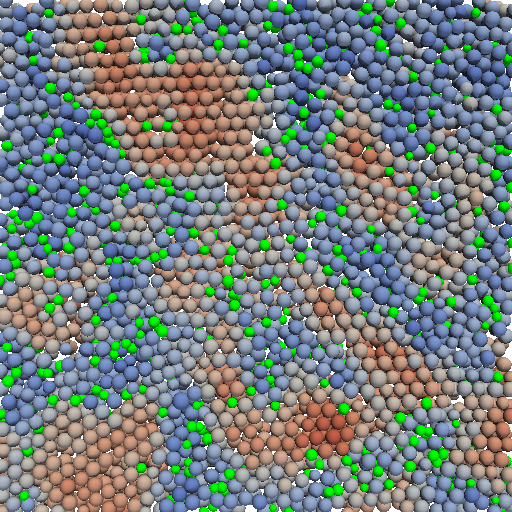
\includegraphics[width=0.29\columnwidth]{small_boo120.png}\\
			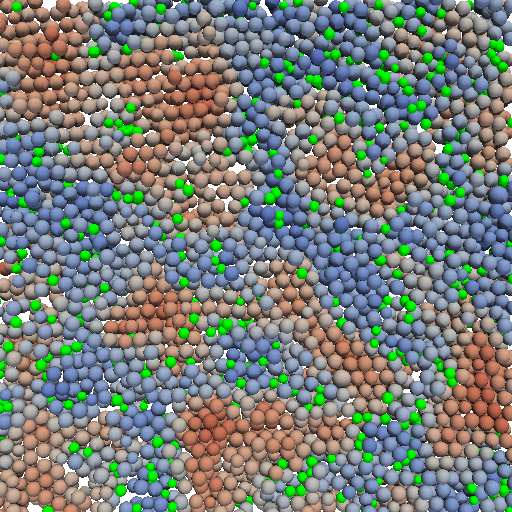
\includegraphics[width=0.29\columnwidth]{small_boo180.png} & %
			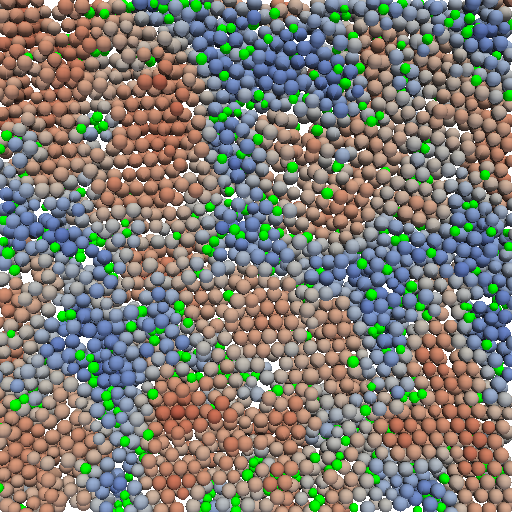
\includegraphics[width=0.29\columnwidth]{small_boo240.png} & %
			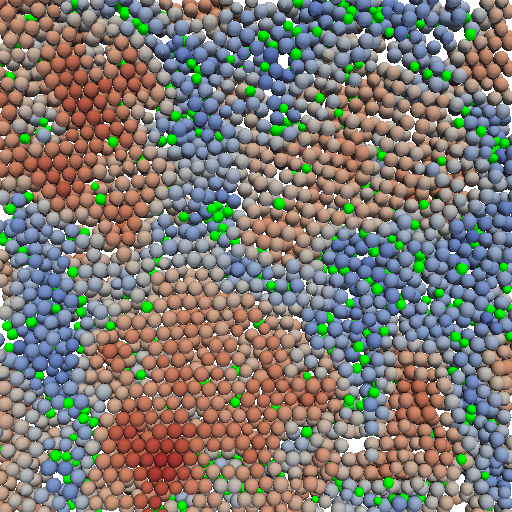
\includegraphics[width=0.29\columnwidth]{small_boo299.png}\\%
		};
		\begin{axis}[%
		name=b,
		at={(a.south east)},%
		anchor=below south west,%
		xmin=0,xmax=10, ymin=0, ymax=0.55,%
		width=0.2\columnwidth,%
		height=0.7\columnwidth,%
		axis x line=none,%
		axis y line*=right,%
		axis on top,
		%title=$Q_6$,%
		%title style={at={(1,1)}}
		]
		\addplot graphics[xmin=0,xmax=10, ymin=0, ymax=0.55] {color_bar.png};
		\end{axis}
		\node[above= 0 of b.outer north] {$Q_6$};
	\end{tikzpicture}
	\caption{\textbf{Heterogeneous nucleation.} Successive computer reconstruction of the first three layers from the wall, every \unit{12}{\hour}, seen from the fluid side. Particles sizes are according to our method. Small ($R<\unit{1.5}{\micro\metre}$) particles are shown in green. Other particles are coloured according to their crystal-like order. Note how the small particles are expelled from the forming crystallites to concentrate in the grain boundaries.}
	\label{fig:small_expelled}
\end{figure}

\tikzset{external/force remake=false}
\tikzsetnextfilename{profiles}
\begin{figure}
	\centering
	\begin{tikzpicture}[
		lab/.style={above right, text height=0.8em, text depth=0.2em, font=\Large\bfseries}%
		]%
		\begin{groupplot}[%
			group style={
				group size=2 by 2,
				y descriptions at=edge left,%
				x descriptions at=edge bottom,%
				horizontal sep=0,
				vertical sep=0,
			},%
			width=0.6\columnwidth,
			height=0.5\columnwidth,%
			ymin=0, ymax=1,%
			ytick={0,0.2,...,1},%
			no marks,%
			ylabel near ticks,%
			xlabel=$z/(2R_\text{peak})$,%
			xmin=1, xmax=26,%
			axis on top,
			]
		\nextgroupplot[ylabel={$\rho$}]
		\addplot+[gray!50, fill=gray!50] table[x index=0, y index=1]{large_small_mrco_t000.gauss.zhist} \closedcycle;
		\addplot+[dashed] table[x index=0, y index=3]{large_small_mrco_t000.gauss.zhist};
		\addplot+[black] table[x index=0, y index=1]{large_small_mrco_t000.zhist};
		\node at (rel axis cs:0.5, 0.8) {$t=0$};
		
		\nextgroupplot
		\addplot+[gray!50, fill=gray!50] table[x index=0, y index=1]{large_small_mrco_t200.gauss.zhist} \closedcycle;
		\addplot+[dashed] table[x index=0, y index=3]{large_small_mrco_t200.gauss.zhist};
		\addplot+[black] table[x index=0, y index=1]{large_small_mrco_t200.zhist};
		\node at (rel axis cs:0.5, 0.8) {$t=\unit{40}{\hour}$};
		
		\nextgroupplot[ymax=0.15, ytick={0,0.1}, ylabel={$\rho$}]
		\addplot+[gray!50, fill=gray!50] table[x index=0, y index=2]{large_small_mrco_t000.gauss.zhist} \closedcycle;
		\addplot+[dashed] table[x index=0, y index=3]{large_small_mrco_t000.gauss.zhist} ;
		\addplot+[black] table[x index=0, y index=2]{large_small_mrco_t000.zhist};
		
		\nextgroupplot[ymax=0.15, ytick={0,0.1}]
		\addplot+[gray!50, fill=gray!50] table[x index=0, y index=2]{large_small_mrco_t200.gauss.zhist} \closedcycle;
		\addplot+[dashed] table[x index=0, y index=3]{large_small_mrco_t200.gauss.zhist};
		\addplot+[black] table[x index=0, y index=2]{large_small_mrco_t200.zhist};
		\end{groupplot}
	\end{tikzpicture}
	\caption{\textbf{Instantaneous density profiles} at $t=0$ (left) and $t=\unit{40}{\hour}$ (right). Top: large particles ($R>\unit{1.5}{\micro\metre}$) without smoothing (black line) and with a Gaussian smoothing of width $2R_\text{peak}$ (gray area). Bottom: small particles ($R<\unit{1.5}{\micro\metre}$) with the same color code. The red curve is the smoothed density of ordered particles ($Q_6>0.25$) irrespective of their size.}
	\label{fig:profiles}
\end{figure}

\tikzset{external/force remake=false}
\tikzsetnextfilename{mrco_ico_small}
\begin{figure}
	\centering
	\begin{tikzpicture}
		\node[anchor=south east] {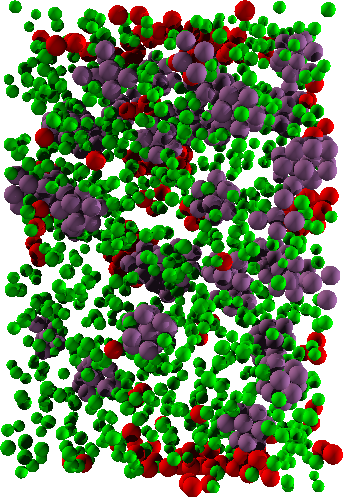
\includegraphics[width=0.45\columnwidth]{mrco_ico_small_t000.png}};
		\node[anchor=south west] {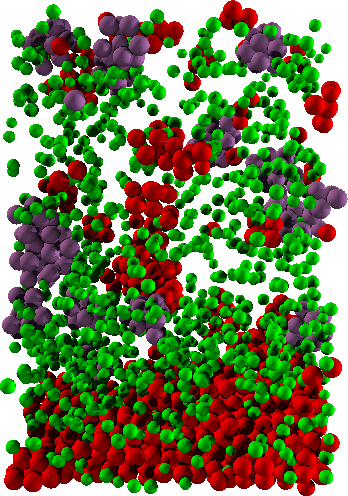
\includegraphics[width=0.45\columnwidth]{mrco_ico_small_t299.png}};
		\draw[->] (0,0.1\columnwidth) -- (0,0.5\columnwidth) node[above]{$z$};
	\end{tikzpicture}
	\caption{\textbf{Structure visualisation} at $t=0$ (left) and $t=\unit{40}{\hour}$ (right). Small particles ($R<\unit{1.5}{\micro\metre}$) are shown in green, crystal-like ordered particles ($Q_6>0.25$) in red and icosahedral particles and their neighbours in purple. Other particles are not shown.}
	\label{fig:mrco_ico_small}
\end{figure}

\end{document}